\documentclass[border=10pt]{standalone}
\usepackage[utf8]{inputenc}
\usepackage{tikz}
\usetikzlibrary{shapes.geometric, arrows.meta}

\tikzset{
  entita/.style    = {rectangle, draw, thick, fill=blue!8, minimum width=20mm, minimum height=8mm, font=\scriptsize, inner sep=2pt},
  debole/.style    = {entita, double, double distance=1.3pt},
  rel/.style       = {diamond, draw, thick, fill=orange!15, aspect=2, inner sep=0pt, minimum width=11mm, minimum height=6mm, font=\tiny},
  c/.style         = {font=\tiny, fill=white, inner sep=0.8pt},
  l/.style         = {thick},
  isa/.style       = {thick, -{Triangle[open, length=3mm, width=4mm]}}
}

\begin{document}
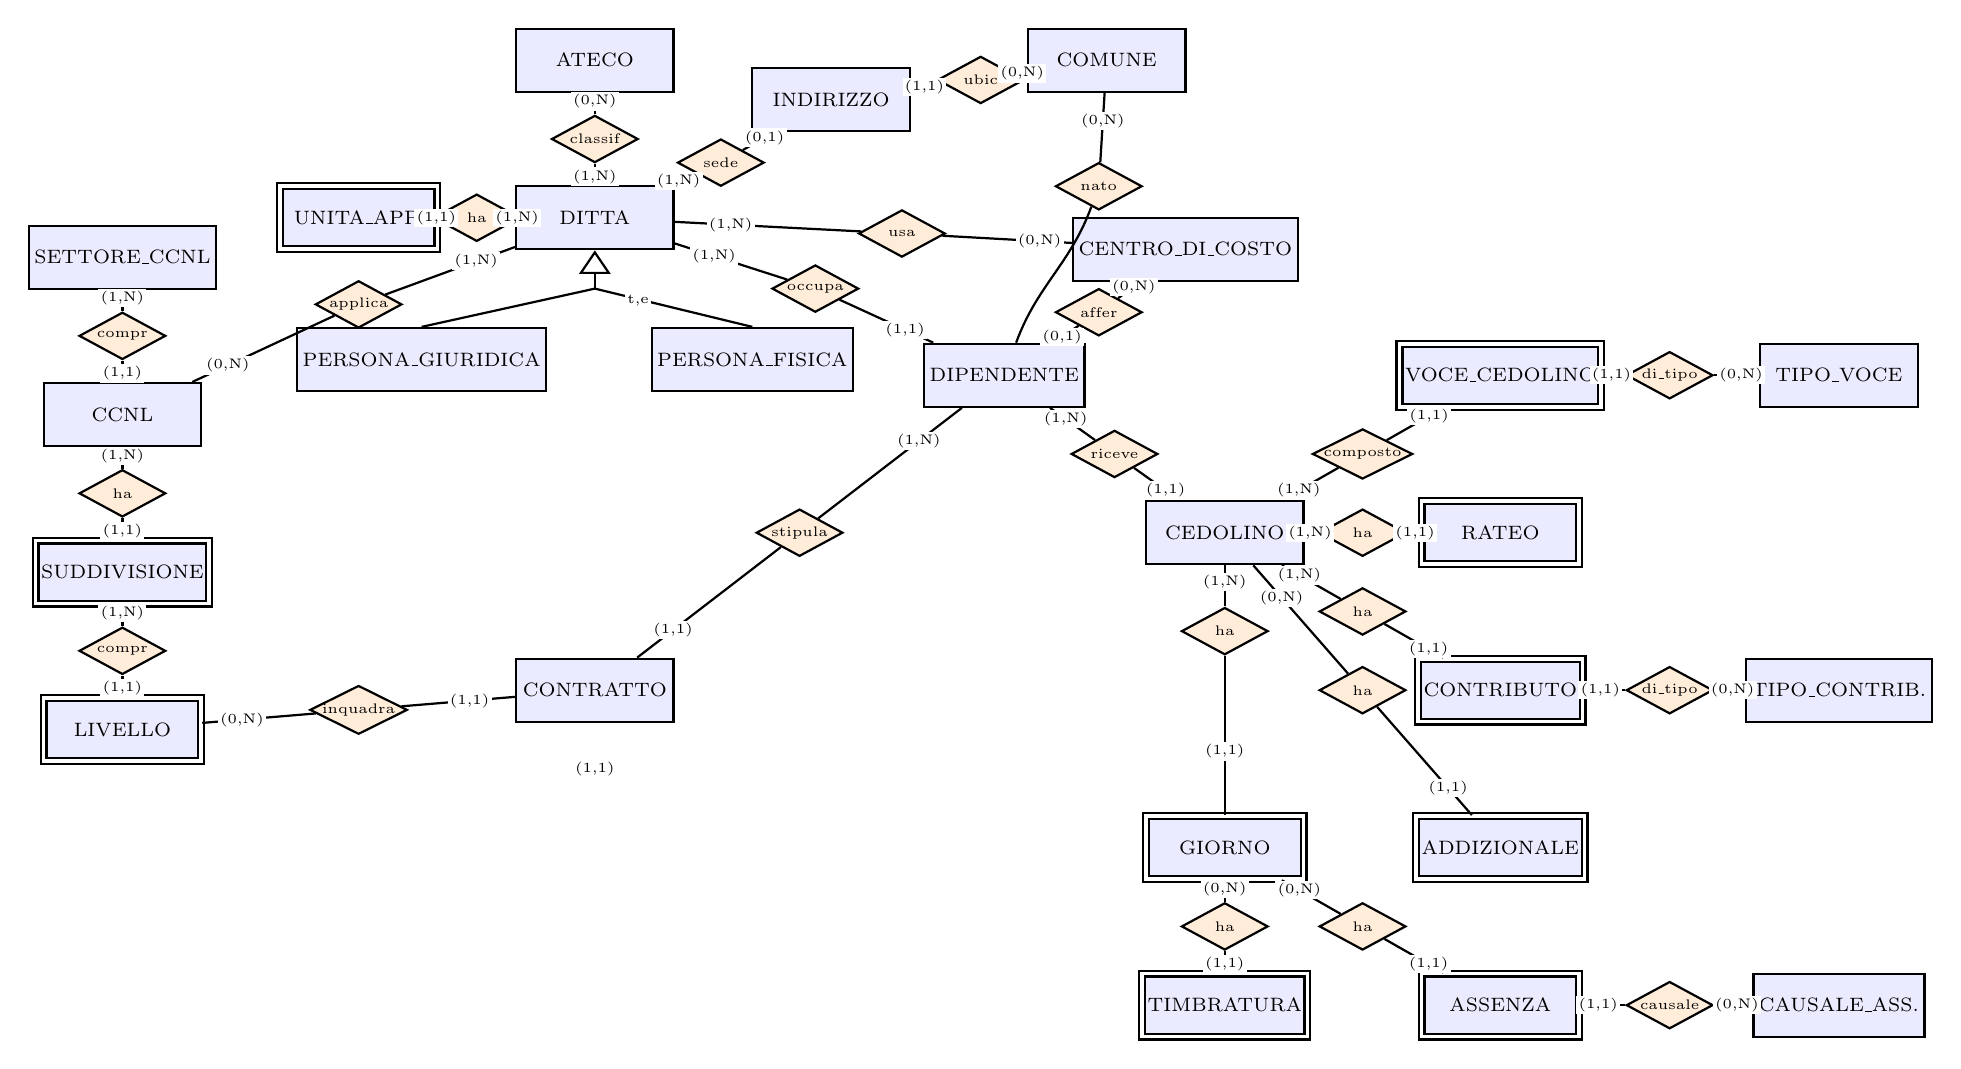
\begin{tikzpicture}[x=1cm, y=1cm]

  % gerarchia contratto collettivo (sinistra)
  \node[entita] (set)  at (-6, 6.5) {SETTORE\_CCNL};
  \node[entita] (ccnl) at (-6, 4.5) {CCNL};
  \node[debole] (sud)  at (-6, 2.5) {SUDDIVISIONE};
  \node[debole] (liv)  at (-6, 0.5) {LIVELLO};

  % ditta e satelliti
  \node[entita] (ditta) at (0, 7.0) {DITTA};
  \node[entita] (ate)  at (0, 9.0) {ATECO};
  \node[debole] (uni)  at (-3, 7.0) {UNITA\_APP.};
  \node[entita] (ind)  at (3, 8.5) {INDIRIZZO};
  \node[entita] (com)  at (6.5, 9.0) {COMUNE};
  \node[entita] (cdc)  at (7.5, 6.6) {CENTRO\_DI\_COSTO};

  % generalizzazione SOTTO la ditta
  \node[entita] (pg) at (-2.2, 5.2) {PERSONA\_GIURIDICA};
  \node[entita] (pf) at (2.0, 5.2) {PERSONA\_FISICA};

  \node[entita] (dip)  at (5.2, 5.0) {DIPENDENTE};
  \node[entita] (con)  at (0, 1.0) {CONTRATTO};
  \node[entita] (ced)  at (8, 3.0) {CEDOLINO};

  % dettaglio cedolino
  \node[debole] (voce) at (11.5, 5.0) {VOCE\_CEDOLINO};
  \node[entita] (tv)   at (15.8, 5.0) {TIPO\_VOCE};
  \node[debole] (rat)  at (11.5, 3.0) {RATEO};
  \node[debole] (contr) at (11.5, 1.0) {CONTRIBUTO};
  \node[entita] (tc)   at (15.8, 1.0) {TIPO\_CONTRIB.};
  \node[debole] (add)  at (11.5,-1.0) {ADDIZIONALE};

  % presenze
  \node[debole] (gio)  at (8,-1.0) {GIORNO};
  \node[debole] (tim)  at (8,-3.0) {TIMBRATURA};
  \node[debole] (ass)  at (11.5,-3.0) {ASSENZA};
  \node[entita] (cau)  at (15.8,-3.0) {CAUSALE\_ASS.};

  % ---------------- GENERALIZZAZIONE ----------------
  \coordinate (fk) at (0,6.1);
  \draw[isa] (fk) -- (ditta.south);
  \draw[l] (pg.north) -- (fk);
  \draw[l] (pf.north) -- (fk);
  \node[c] at (0.55,5.95) {t,e};

  % ---------------- RELAZIONI ----------------
  \node[rel] (r1) at (-6,5.5) {compr}; \draw[l] (set)--(r1) node[c,pos=.4]{(1,N)}; \draw[l] (r1)--(ccnl) node[c,pos=.6]{(1,1)};
  \node[rel] (r2) at (-6,3.5) {ha};    \draw[l] (ccnl)--(r2) node[c,pos=.4]{(1,N)}; \draw[l] (r2)--(sud) node[c,pos=.6]{(1,1)};
  \node[rel] (r3) at (-6,1.5) {compr}; \draw[l] (sud)--(r3) node[c,pos=.4]{(1,N)}; \draw[l] (r3)--(liv) node[c,pos=.6]{(1,1)};

  \node[rel] (r4) at (-1.5,7.0) {ha};    \draw[l] (uni)--(r4) node[c,pos=.35]{(1,1)}; \draw[l] (r4)--(ditta) node[c,pos=.65]{(1,N)};
  \node[rel] (r5) at (0,8.0) {classif};  \draw[l] (ditta)--(r5) node[c,pos=.4]{(1,N)}; \draw[l] (r5)--(ate) node[c,pos=.6]{(0,N)};
  \node[rel] (r6) at (1.6,7.7) {sede};   \draw[l] (ditta)--(r6) node[c,pos=.35]{(1,N)}; \draw[l] (r6)--(ind) node[c,pos=.7]{(0,1)};
  \node[rel] (r7) at (4.9,8.75) {ubic};  \draw[l] (ind)--(r7) node[c,pos=.4]{(1,1)}; \draw[l] (r7)--(com) node[c,pos=.6]{(0,N)};
  \node[rel] (r8) at (3.9,6.8) {usa};    \draw[l] (ditta)--(r8) node[c,pos=.3]{(1,N)}; \draw[l] (r8)--(cdc) node[c,pos=.75]{(0,N)};

  \node[rel] (r9) at (-3,5.9) {applica}; \draw[l] (ditta)--(r9) node[c,pos=.3]{(1,N)}; \draw[l] (r9)--(ccnl) node[c,pos=.75]{(0,N)};

  \node[rel] (r10) at (2.8,6.1) {occupa}; \draw[l] (ditta)--(r10) node[c,pos=.35]{(1,N)}; \draw[l] (r10)--(dip) node[c,pos=.7]{(1,1)};
  \node[rel] (r11) at (6.4,5.8) {affer};  \draw[l] (dip)--(r11) node[c,pos=.35]{(0,1)}; \draw[l] (r11)--(cdc) node[c,pos=.7]{(0,N)};
  \node[rel] (r12) at (6.4,7.4) {nato};   \draw[l] (dip) to[out=70,in=250] (r12) node[c,pos=.7]{(1,1)}; \draw[l] (r12)--(com) node[c,pos=.6]{(0,N)};
  \node[rel] (r13) at (2.6,3.0) {stipula};\draw[l] (dip)--(r13) node[c,pos=.3]{(1,N)}; \draw[l] (r13)--(con) node[c,pos=.75]{(1,1)};
  \node[rel] (r14) at (-3,0.75) {inquadra};\draw[l] (con)--(r14) node[c,pos=.4]{(1,1)}; \draw[l] (r14)--(liv) node[c,pos=.65]{(0,N)};
  \node[rel] (r15) at (6.6,4.0) {riceve}; \draw[l] (dip)--(r15) node[c,pos=.35]{(1,N)}; \draw[l] (r15)--(ced) node[c,pos=.7]{(1,1)};

  \node[rel] (r16) at (9.75,4.0) {composto}; \draw[l] (ced)--(r16) node[c,pos=.3]{(1,N)}; \draw[l] (r16)--(voce) node[c,pos=.75]{(1,1)};
  \node[rel] (r17) at (13.65,5.0){di\_tipo}; \draw[l] (voce)--(r17) node[c,pos=.4]{(1,1)}; \draw[l] (r17)--(tv) node[c,pos=.6]{(0,N)};
  \node[rel] (r18) at (9.75,3.0) {ha};       \draw[l] (ced)--(r18) node[c,pos=.4]{(1,N)}; \draw[l] (r18)--(rat) node[c,pos=.6]{(1,1)};
  \node[rel] (r19) at (9.75,2.0) {ha};       \draw[l] (ced)--(r19) node[c,pos=.3]{(1,N)}; \draw[l] (r19)--(contr) node[c,pos=.75]{(1,1)};
  \node[rel] (r20) at (13.65,1.0){di\_tipo}; \draw[l] (contr)--(r20) node[c,pos=.4]{(1,1)}; \draw[l] (r20)--(tc) node[c,pos=.6]{(0,N)};
  \node[rel] (r21) at (9.75,1.0) {ha};       \draw[l] (ced)--(r21) node[c,pos=.3]{(0,N)}; \draw[l] (r21)--(add) node[c,pos=.75]{(1,1)};

  \node[rel] (r22) at (8,1.75) {ha};         \draw[l] (ced)--(r22) node[c,pos=.4]{(1,N)}; \draw[l] (r22)--(gio) node[c,pos=.6]{(1,1)};
  \node[rel] (r23) at (8,-2.0) {ha};         \draw[l] (gio)--(r23) node[c,pos=.4]{(0,N)}; \draw[l] (r23)--(tim) node[c,pos=.6]{(1,1)};
  \node[rel] (r24) at (9.75,-2.0) {ha};      \draw[l] (gio)--(r24) node[c,pos=.3]{(0,N)}; \draw[l] (r24)--(ass) node[c,pos=.75]{(1,1)};
  \node[rel] (r25) at (13.65,-3.0){causale}; \draw[l] (ass)--(r25) node[c,pos=.4]{(1,1)}; \draw[l] (r25)--(cau) node[c,pos=.6]{(0,N)};

\end{tikzpicture}
\end{document}
